\documentclass[aspectratio=169]{beamer}
\usetheme{Madrid}
\usecolortheme{seahorse}
\setbeamertemplate{navigation symbols}{}
\usepackage[T1]{fontenc}
\usepackage[utf8]{inputenc}
\usepackage{lmodern}
\usepackage{graphicx}
\graphicspath{{../assets/figures/}{../../reports/publication/}}

\title{ORIUS in One View}
\subtitle{A Safety Layer for Physical AI}
\author{Pratik Niroula}
\date{April 2026}

\begin{document}

\begin{frame}
  \titlepage
\end{frame}

\begin{frame}{Why ORIUS Exists}
  \begin{itemize}
    \item Physical AI can look safe in observed state while violating the true state of the plant.
    \item ORIUS is built to close that hidden observability gap online.
    \item The core runtime loop is Detect, Calibrate, Constrain, Shield, and Certify.
  \end{itemize}
\end{frame}

\begin{frame}{Architecture}
  \centering
  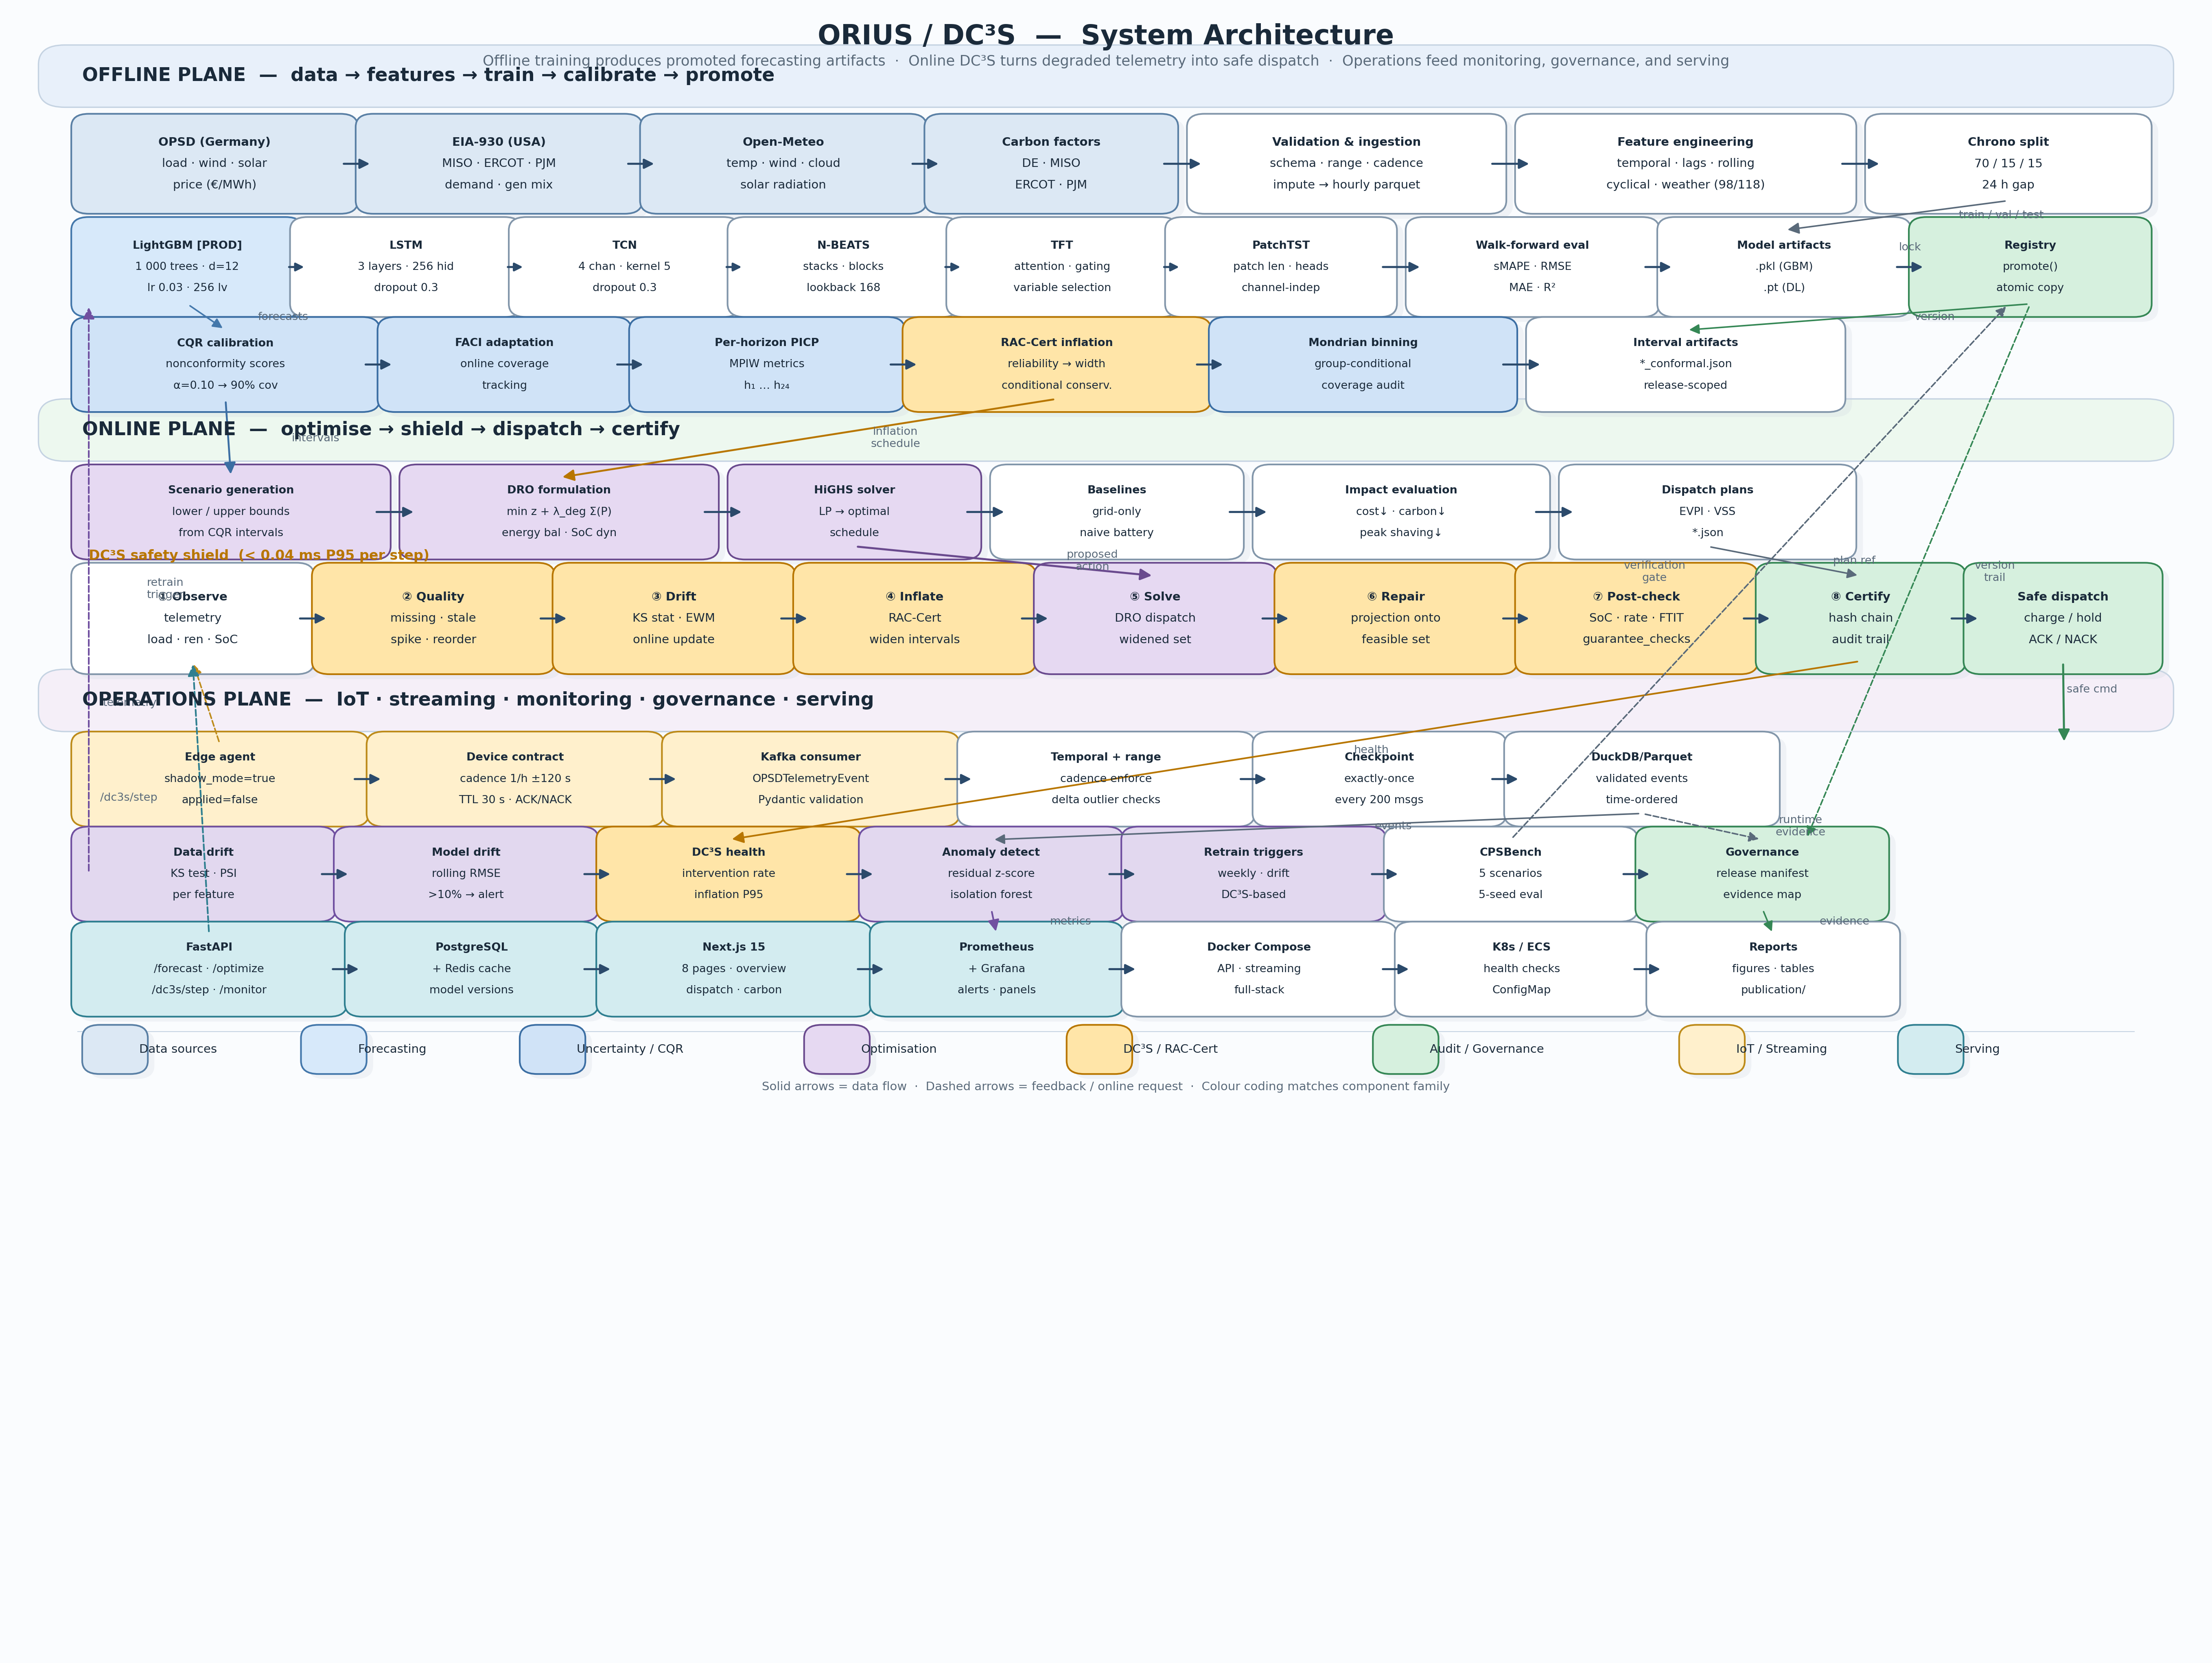
\includegraphics[width=0.95\textwidth]{fig01_architecture.png}
\end{frame}

\begin{frame}{How the Book Is Organized}
  \centering
  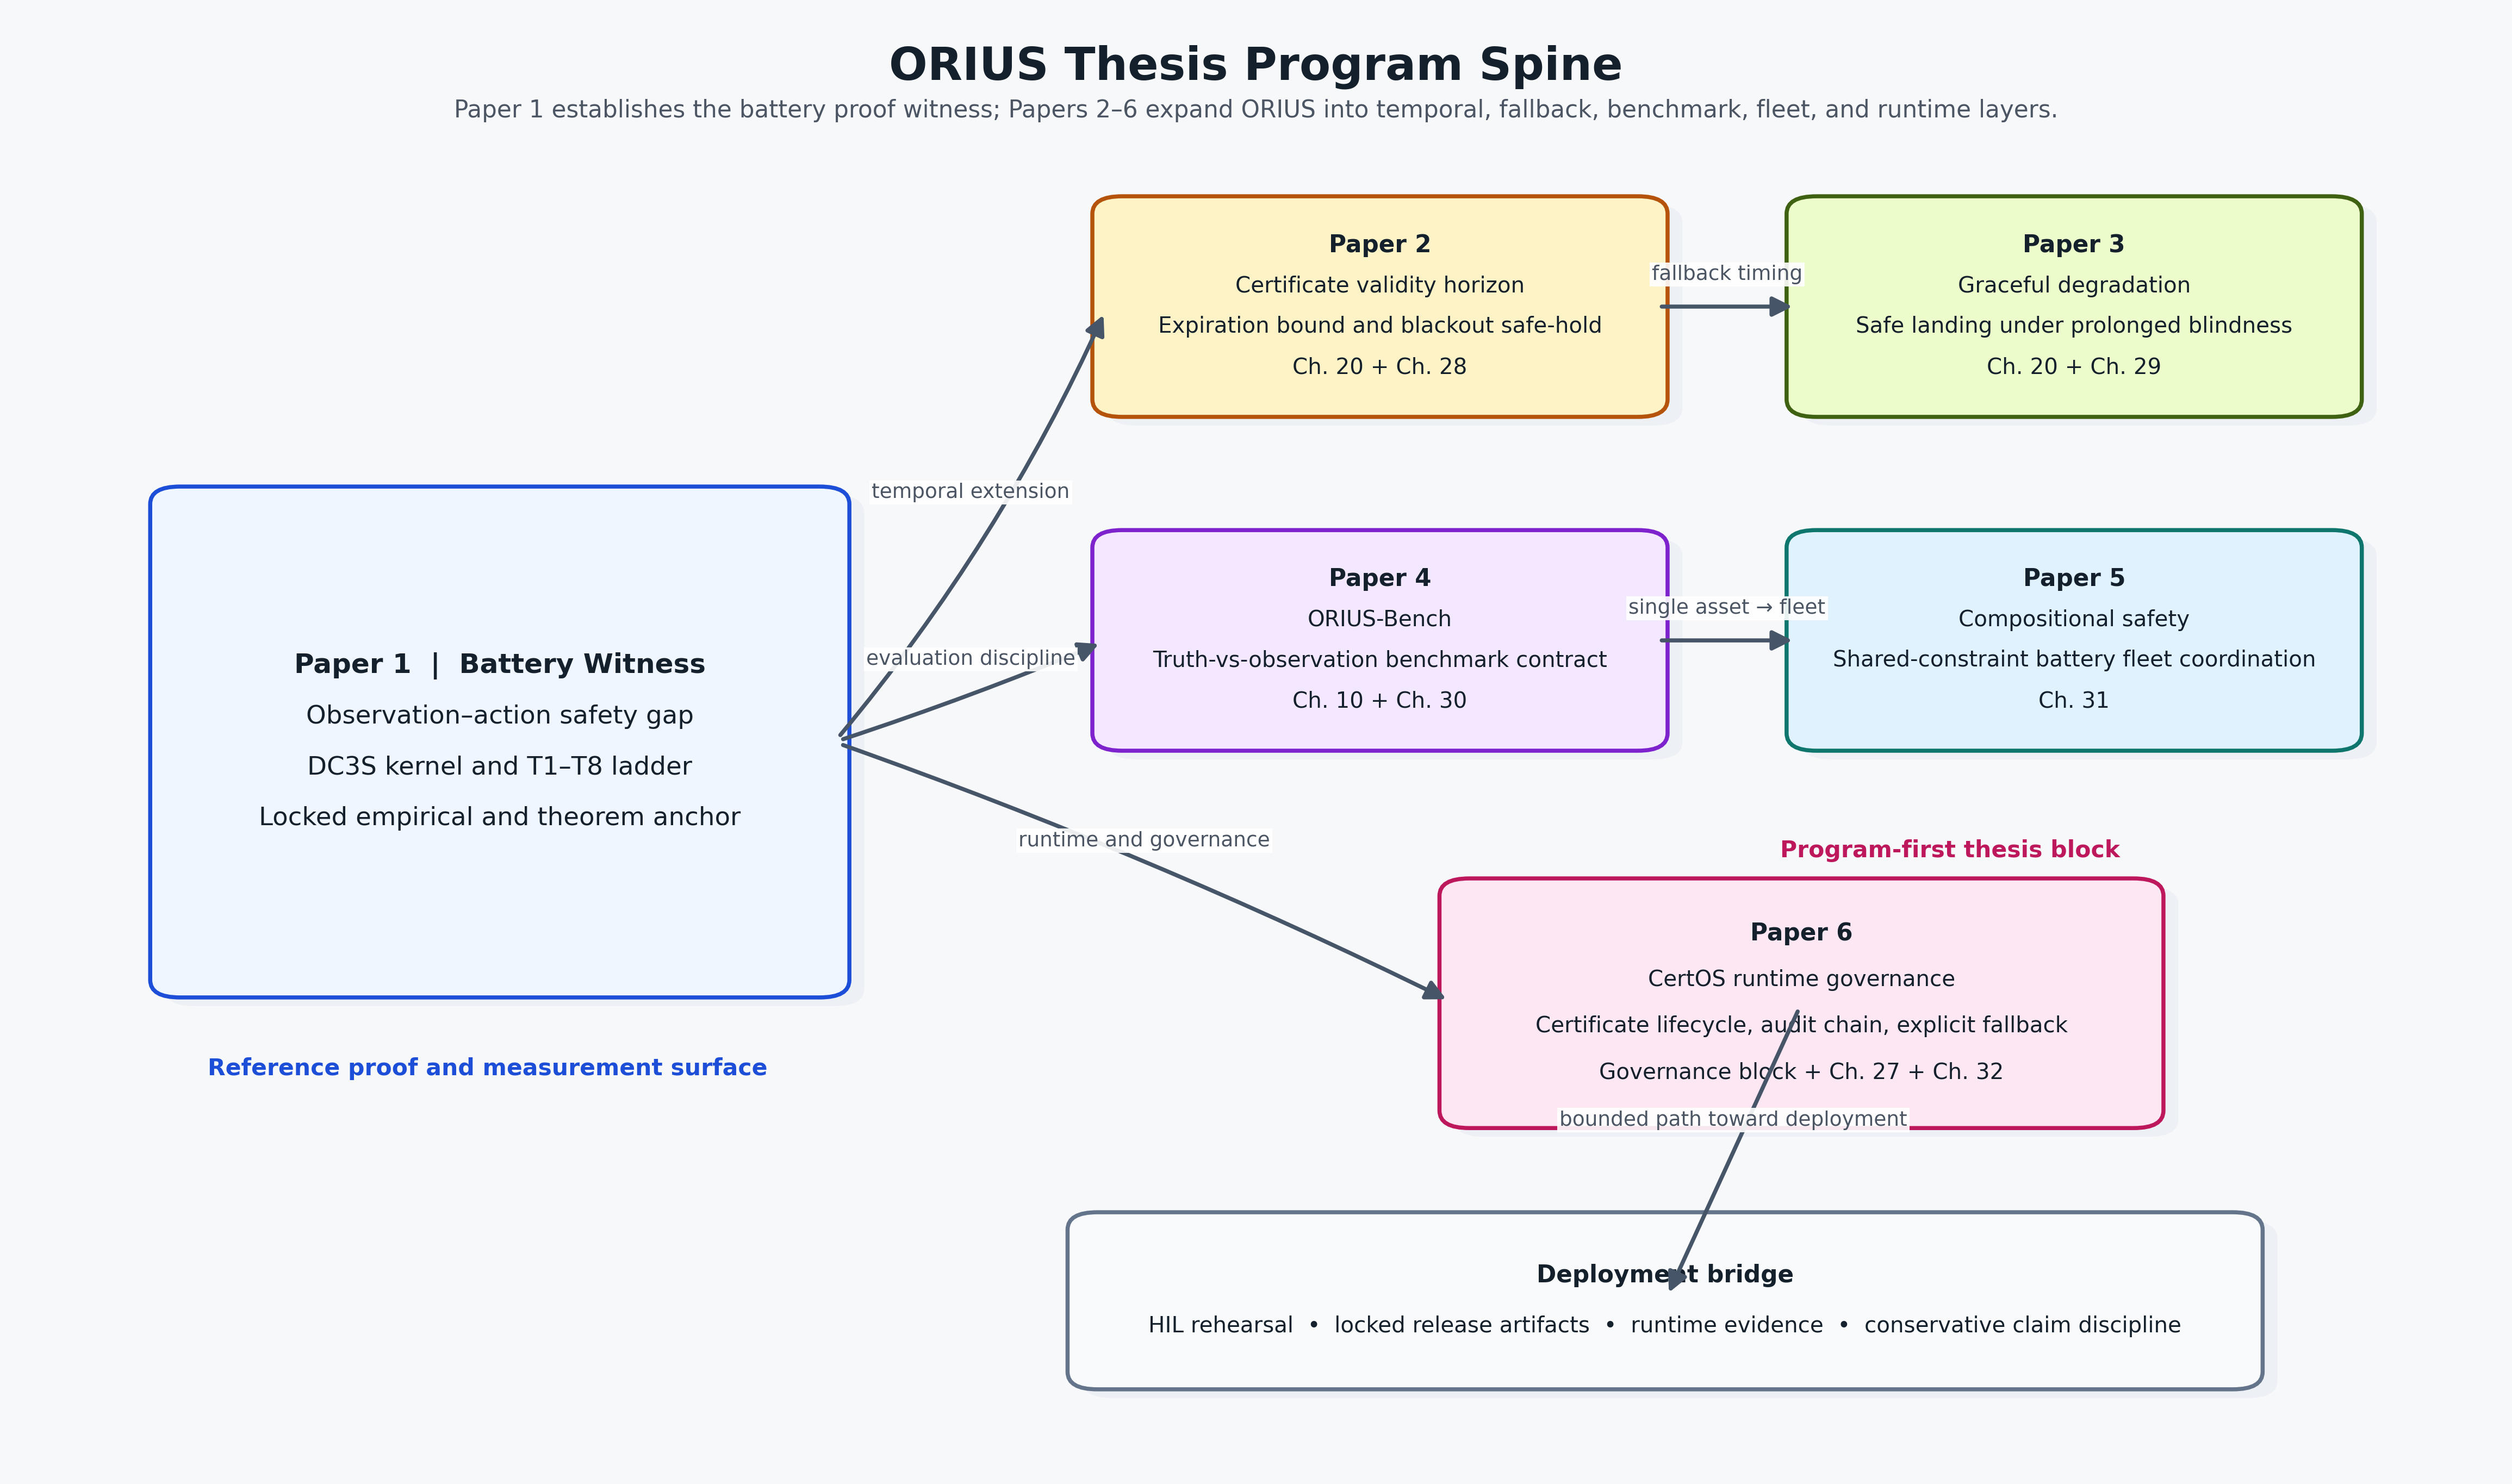
\includegraphics[width=0.88\textwidth]{fig46_orius_program_spine.png}
\end{frame}

\begin{frame}{Six-Domain Scope}
  \centering
  
\includegraphics[width=0.98\textwidth]{fig_orius_theory_runtime_domain_flow.png}
\end{frame}

\begin{frame}{Current Evidence Status}
  \centering
  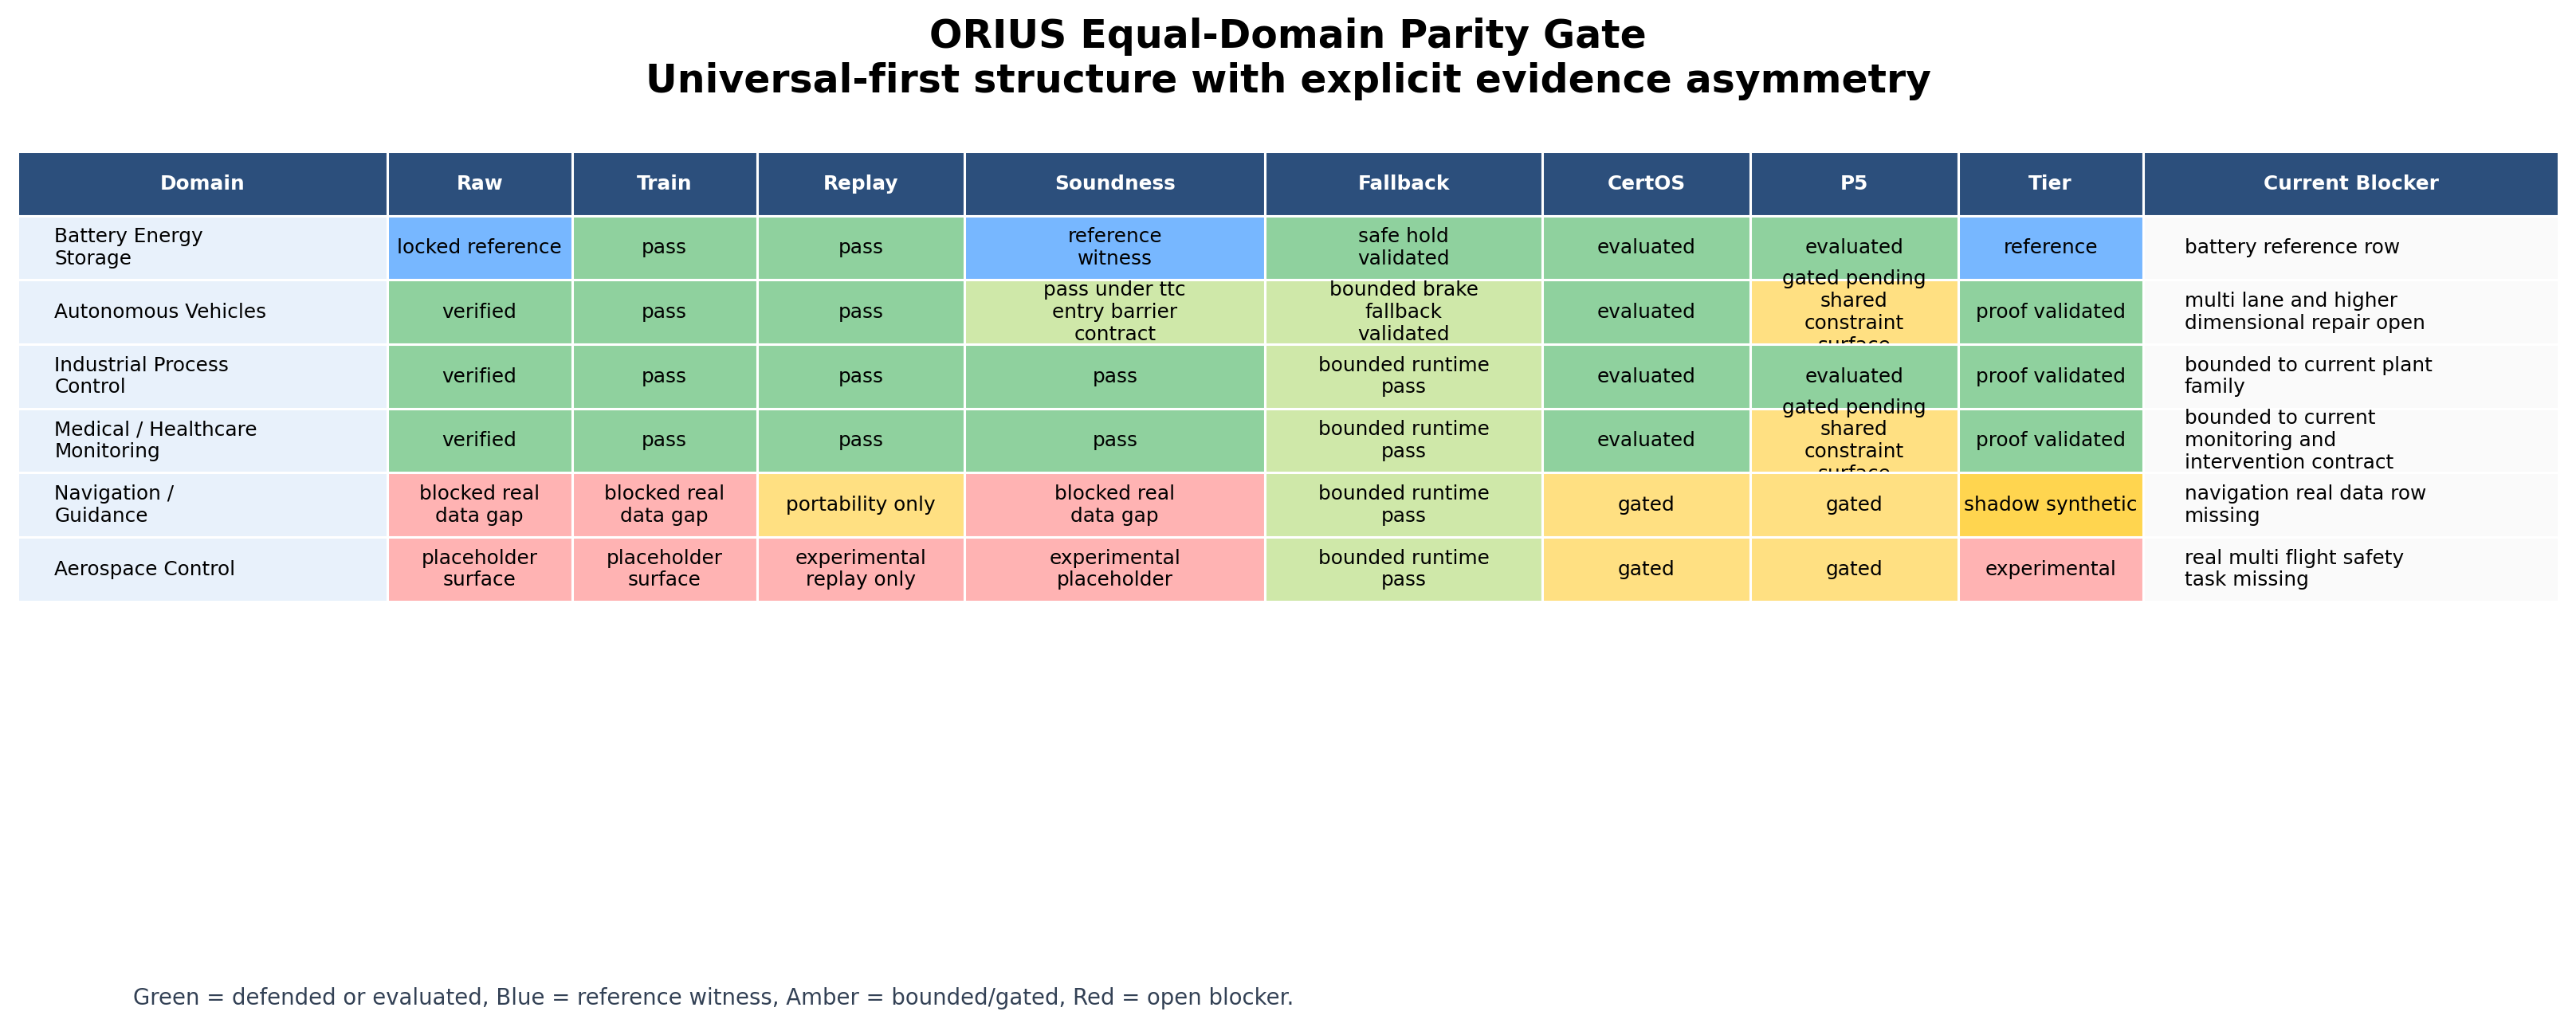
\includegraphics[width=\textwidth]{fig_orius_equal_domain_parity_matrix.png}
\end{frame}

\begin{frame}{What the Monograph Can Claim Today}
  \begin{itemize}
    \item Battery is the deepest reference witness.
    \item Industrial, healthcare, and bounded AV rows are defended.
    \item Navigation and aerospace are still explicit open gates.
    \item The book is universal-first in structure and conservative in evidence.
  \end{itemize}
\end{frame}

\begin{frame}{Deliverables}
  \begin{itemize}
    \item 455-page book-length PDF
    \item 183-reference bibliography
    \item five-reviewer R1-style dossier
    \item parity matrix and governed claim surface
  \end{itemize}
\end{frame}

\end{document}
